\documentclass{beamer}

\usepackage[utf8]{inputenc} % For encoding
\usepackage{graphicx}
\usepackage{amsmath}
\usepackage{amssymb}
\usepackage{makecell}

\usepackage[T1]{fontenc}
\usepackage{booktabs}
\usepackage{multicol}
\usepackage{natbib}
\usepackage{hyperref}
\usepackage{booktabs} % For professional quality tables
\usepackage{array}    % For better column alignment
\usepackage{tabularx}
\usepackage{tikz}

\usepackage{pgfkeys}
\usepackage{ifthen}

% \usepackage[a4paper,width=175mm,top=20mm,bottom=20mm,bindingoffset=6mm]{geometry}
\usepackage{fancyhdr}

\title{Maintenance Scheduling System}
\author{Christian Brunbjerg Jespersen}
\institute{Technical University of Denmark}
\date{\today}

\usepackage{fontspec}

% Set the main document font to Arial
\setmainfont{FiraCode Nerd Font}
\begin{document}

% Sets
\newcommand{\SetWorkOrder}[1]{W(\VarMetaTime, \VarStrategicWorkOrderAssignment{}{})}
\newcommand{\SetPeriod}{P(\VarMetaTime)}
\newcommand{\SetResource}{R(\VarMetaTime)} %RECONSIDER | RELEVANT FOR BOTH STRATEGIC AND TACTICAL
\newcommand{\SetOperation}[2]{O_{#1}(\VarMetaTime, #2 )}

\newcommand{\SetDays}[1]{D_{#1}(\VarMetaTime)}
\newcommand{\SetActivity}[2]{A_{#2}(\VarMetaTime, #1)}
\newcommand{\SetTechnician}{T(\VarMetaTime)}
\newcommand{\SetWorkSegment}{K(\VarSupervisorAssignment{}{})}

\newcommand{\SetTimeInstance}{I(\VarMetaTime)}
\newcommand{\SetEvent}{E(\VarMetaTime)}

% Parameters
\newcommand{\ParStrategicValue}{strategic\_value_{wp}(\VarMetaTime)}
\newcommand{\ParStrategicPenalty}{strategic\_penalty}
\newcommand{\ParClusteringValue}{clustering\_value_{w1, w2}}
\newcommand{\ParStrategicResource}{resource_{pr}(\VarMetaTime)}

\newcommand{\ParStrategicWorkOrderWeight}{work\_order\_work_{wr}}
\newcommand{\ParStrategicInclude}{include(\VarMetaTime)}
\newcommand{\ParStrategicExclude}{exclude(\VarMetaTime)}
\newcommand{\ParTacticalValue}{tactical\_value_{do}(\VarMetaTime)}

\newcommand{\ParTacticalPenalty}{tactical\_penalty}
\newcommand{\ParOperationWork}[1]{work_{#1}(\VarMetaTime)}
\newcommand{\ParTacticalResource}{tactical\_resource_{dr}(\VarMetaTime)}
\newcommand{\ParStartStart}{start\_start_{o1, o2}}

\newcommand{\ParFinishStart}{finish\_start_{o1, o2}}
\newcommand{\ParNumberOfPeople}{number_{o}(\VarMetaTime)}
\newcommand{\ParOperatingTime}{operating\_time_{o}}
\newcommand{\ParDurationLower}{duration\_lower_{o}(\VarMetaTime)}

\newcommand{\ParDurationUpper}{duration\_upper_{o}(\VarMetaTime)}
\newcommand{\ParSupervisorValue}{supervisor\_value_{at}(\VarMetaTime)} % We should determine if the supervisor should assign for each operation or for each activity. My guts say that it should be for each activity
\newcommand{\ParFeasible}{feasible_{at}(\VarIncludeActivity{})}
\newcommand{\ParOperationsForWorkOrder}{work\_order\_to\_operations_{w}}

\newcommand{\ParOperationsInWorkOrder}{operations\_in\_work\_order_{w}}
\newcommand{\ParActivitiesForOperation}{activities\_for\_operation_{o}}
\newcommand{\ParLowerActivityWork}{lower\_activity\_work_{a}(\VarMetaTime)}
\newcommand{\ParActivityWork}[1]{activity\_work_{a}(\VarMetaTime, \VarActivityWork{#1})}
\newcommand{\ParPreparation}{preparation_{a1, a2}}

\newcommand{\ParEvent}{event_{ie}}
\newcommand{\ParEventDuration}{duration_{ie}}
\newcommand{\ParConstraintLimit}{constraint\_limit}
\newcommand{\ParTimeWindowStart}{time\_window\_start_{a}(\VarTacticalWork{}{})}

\newcommand{\ParTimeWindowFinish}{time\_window\_finish_{a}(\VarTacticalWork{}{})}
\newcommand{\ParAvailabilityStart}{availability\_start(\VarMetaTime)}
\newcommand{\ParAvailabilityFinish}{availability\_finish(\VarMetaTime)}

% Variables
\newcommand{\VarStrategicWorkOrderAssignment}[2]{\alpha_{#1#2}(\VarMetaTime)}
\newcommand{\VarStrategicExcess}{\epsilon_{pr}(\VarMetaTime)}
\newcommand{\VarTacticalWork}[2]{\beta_{#1#2}(\VarMetaTime)}
\newcommand{\VarTacticalExcess}{\mu_{rd}(\VarMetaTime)} : excess capacity for each day

\newcommand{\VarTacticalWorkBinary}[2]{\sigma_{#1#2}(\VarMetaTime)}
\newcommand{\VarTacticalWorkBinaryConsecutive}{\eta_{do}(\VarMetaTime)}
\newcommand{\VarTacticalOperationDifference}{\Delta_{o}(\VarMetaTime)}
\newcommand{\VarSupervisorAssignment}[2]{\gamma_{#1#2}(\VarMetaTime)}
\newcommand{\VarSupervisorAssignmentWhole}{\phi_{o}(\VarMetaTime)}

\newcommand{\VarActivityWork}[1]{\rho_{#1}(\VarMetaTime)}

\newcommand{\VarProcessingTime}{\delta_{ak}(\VarMetaTime)} 
\newcommand{\VarActiveSegment}[2]{\pi_{#1#2}(\VarMetaTime)}
\newcommand{\VarStartOfSegment}[2]{\lambda_{#1#2}(\VarMetaTime)}
\newcommand{\VarFinishOfSegment}[2]{\Lambda_{#1#2}(\VarMetaTime)}

\newcommand{\VarSegmentInRelation}{\omega_{akie}(\VarMetaTime)}
\newcommand{\VarIncludeActivity}[1]{\theta_{#1}(\VarMetaTime)}

% Meta variables
\newcommand{\VarMetaTime}{\tau}

\usetikzlibrary {positioning}


\definecolor{red}{HTML}{8A3F3A}
\definecolor{yellow}{HTML}{E0BB3C}
\definecolor{blue}{HTML}{4569E0}
\definecolor{green}{HTML}{17E561}
\definecolor{other}{HTML}{6A939E}

\newcommand{\ModelColor}{red}
\newcommand{\UserInterfaceColor}{yellow}
\newcommand{\PersistenceColor}{blue}
\newcommand{\PointerSwapColor}{green}
\newcommand{\OrchestratorColor}{other}

\pgfkeys{
	/graph/.is family, /graph,
	default/.style = {
		show_shared_pointer = false,
		show_orchestrator = false,
		show_persistence = false,
		show_user_interface = false,
		basis/.estore in = 2cm,
	},
	show_shared_pointer/.estore in = \ShowSharedSolutionCommunication,
	show_orchestrator/.estore in = \ShowOrchestratorCommunication,
	show_persistence/.estore in = \ShowPersistenceCommunication,
	show_user_interface/.estore in = \ShowUserInterfaceCommunication,
	basis/.estore in = \basisinput,
}
\newlength{\basis}
\tikzset{
  basis/.code={\setlength{\basis}{\basisinput}}, % TikZ assignment code
  basis/.default=1cm,                   % Provide a default (\b@sis is undefined/unassigned)
  basis,                                % Set initial Value (\b@sis is defined/assigned)
 }

\newcommand{\drawGraph}[1]{
	\pgfkeys{/graph, default, #1}
	
	\begin{tikzpicture}[scale=0.75][
		% Define styles and settings
		node distance=2cm,
		block/.style={rectangle, draw, fill=blue!20, text centered, minimum height=3em},
		arrow/.style={-Stealth, thick}
		]


		\ifthenelse{\equal{\ShowOrchestratorCommunication}{true}}{
			\draw[color=other,-, ultra thick] (Strategic) -- (Orchestrator);
			\draw[color=other,-, ultra thick] (Tactical) -- (Orchestrator);
			\draw[color=other,-, ultra thick] (Supervisor) -- (Orchestrator);
			\draw[color=other,-, ultra thick] (Operational_1) -- (Orchestrator);
			\draw[color=other,-, ultra thick] (Operational_2) -- (Orchestrator);
			\draw[color=other,-, ultra thick] (Operational_3) -- (Orchestrator);
		}{}
		% \draw[help lines] (0\basis, 0\basis) grid (10\basis, 8\basis);
		\draw (5\basis,4\basis) node[minimum height=5cm,minimum width=7.0cm,rounded corners=5pt] {};

	    \draw (2.5\basis,5.5\basis) node[minimum height=1cm,minimum width=1cm,fill=\ModelColor,rounded corners=5pt] (Strategic) {Stra};
	    \draw (5.0\basis,4.0\basis) node[minimum height=1cm,minimum width=1\basis,fill=\ModelColor,rounded corners=5pt] (Supervisor) {Sup};
		\draw (7.5\basis,5.5\basis) node[minimum height=1cm,minimum width=1cm,fill=\ModelColor,rounded corners=5pt] (Tactical) {Tac};

		\draw (2.5\basis,2.5\basis) node[minimum height=1cm,minimum width=1cm,fill=\ModelColor,rounded corners=5pt] (Operational_1) {$O_{1}$};
		\draw (5.0\basis,2.5\basis) node[minimum height=1cm,minimum width=1cm,fill=\ModelColor,rounded corners=5pt] (Operational_2) {$O_{2}$};
		\draw (7.5\basis,2.5\basis) node[minimum height=1cm,minimum width=1cm,fill=\ModelColor,rounded corners=5pt,rounded corners=5pt] (Operational_3) {$O_{3}$};
	
		\draw (Strategic) edge (Tactical);
		\draw (Strategic) edge (Tactical);
		\draw (5\basis,5.5\basis) edge (Supervisor);
		\draw (Supervisor) edge (Operational_1);
		\draw (Supervisor) edge (Operational_2);
		\draw (Supervisor) edge (Operational_3);
		\draw (5.0\basis,0.5\basis)   node[minimum height=1cm,minimum width=5.0cm,            fill=\PersistenceColor,rounded corners=5pt] {SchedulingEnvironment};
		\draw (5.0\basis,7.5\basis)   node[minimum height=1cm,minimum width=5.0cm,            fill=\OrchestratorColor,rounded corners=5pt] (Orchestrator) {Orchestrator};
		\draw (0.5\basis,4.0\basis)   node[rotate=90, minimum height=1cm, minimum width=3.25cm,fill=\PointerSwapColor,rounded corners=5pt] {SharedSolution};
		\draw (9.5\basis,5.5\basis) node[rotate=90, minimum height=1cm, minimum width=1cm,fill=\UserInterfaceColor,rounded corners=5pt] {UI};
		\draw (9.5\basis,4.0\basis)   node[rotate=90, minimum height=1cm, minimum width=1cm,fill=\UserInterfaceColor,rounded corners=5pt] {UI};
		\draw (9.5\basis,2.5\basis) node[rotate=90, minimum height=1cm, minimum width=1cm,fill=\UserInterfaceColor,rounded corners=5pt] {UI};

		% Legend
		\begin{scope}[shift={(10.6\basis,5.7\basis)}]
			\node at (-0.25\basis,1\basis) [right] {Communication Type};
			\draw[color=\OrchestratorColor,fill] (0\basis,0.0\basis) rectangle (0.5cm, 0.5cm);
			\node[anchor=west] at (0.5\basis, 0.25\basis) {\scriptsize Channels};
			\draw[color=\PointerSwapColor,fill] (0\basis,-1.0\basis) rectangle(0.5cm, -0.5cm); 
			\node[anchor=west] at (0.5\basis, -0.75\basis) {\scriptsize Atomic Pointer Swap};
			\draw[color=\ModelColor,fill] (0\basis,-2.0\basis) rectangle(0.5cm, -1.5cm); 
			\node[anchor=west] at (0.5\basis, -1.75\basis) {\scriptsize Metaheurics};
			\draw[color=\PersistenceColor,fill] (0\basis,-3.0\basis) rectangle(0.5cm, -2.5cm); 
			\node[anchor=west] at (0.5\basis, -2.75\basis) {\scriptsize Mutex lock};
			\draw[color=\UserInterfaceColor,fill] (0\basis,-4.0\basis) rectangle(0.5cm, -3.5cm); 
			\node[anchor=west] at (0.5\basis, -3.75\basis) {\scriptsize Channels};
		\end{scope}
		\ifthenelse{\equal{\ShowSharedSolutionCommunication}{true}}{
			\draw[->, thick] (Strategic) -- (Orchestrator);
		}{}
		\ifthenelse{\equal{\ShowUserInterfaceCommunication}{true}}{
			\draw[->, thick] (Strategic) -- (Orchestrator);
		}{}
		\ifthenelse{\equal{\ShowPersistenceCommunication}{true}}{
			\draw[->, thick] (Strategic) -- (Orchestrator);
		}{}
		

	\end{tikzpicture}
}



\frame{\titlepage}
\begin{frame}{Agenda}
    \begin{itemize}
        \item Introduction to Maintenance Scheduling
        \item Architecture of a Scheduling System
        \item Possible Contributions to Operation Research
    \end{itemize}
\end{frame}
\begin{frame}{}
    \begin{block}{Mathematical Notation: Sets }

	\begin{minipage}
		$ a \in A_{b,c}^{m}(t, x, y)$
	\end{minipage}

	\begin{itemize}
		\item a: set element
		\item A: set itself
		\item b: set element from set B
		\item c: set element from set C
		\item m: model formulation m
		\item t: time
		\item x: value of decision variable from a different model
		\item y: value of decision variable from a different model
	\end{itemize}
	
    \end{block}
\end{frame}

\begin{frame}{}
    \begin{block}{Mathematical Notation: Parameters}

	$ name\_of\_parameter_{a, b}(t, x, y) $
	\begin{itemize}
		\item parameters are functions of set elements and input parameters
		\item a: set element from A
		\item b: set element from B
		\item t: time
		\item x: value of decision variable from another model
		\item y: value of decision variable from another model
	\end{itemize}
    \end{block}
\end{frame}

\begin{frame}{}
    \begin{block}{Mathematical Notation: Variables}
	\par
	$ x_{a, b}^{m}(t) $ \\ 
	\begin{itemize}
		\item variables are functions of set elements, specified model, and time
		\item x: decision variable
		\item a: set element from A
		\item b: set element from B
		\item m: specifying the model
		\item t: time
		\item Notice: decision variables cannot depend on other decision variables as it would make them belong to the same model.
	\end{itemize}
    \end{block}
\end{frame}

\begin{frame}[t]{Strategic}
	\scalebox{0.4}{
		\begin{minipage}{2.5\textwidth}
			\section{The Strategic Model}


The Strategic Model have multiple different purposes.
\begin{itemize}
	\item Schedule Work Order out across the weekly periods
	\item Prioritize all the different released work orders
	\item Respect the available weekly hours available for each trait
\end{itemize}

The Strategic model is responsible for grouping work orders into weekly or biweekly periods depending on which kind of maintenance setup that one is running.
This kind of model closely resembles a variant of the multi-compartment multi-knapsack problem. 

\begin{alignat}{2}
	\text{Min} &\sum_{w \in W} \sum_{p \in P} v_{wp}(t) \cdot x_{wp}(t)                                                                                             \\ 
	+ & \sum_{p \in P} \sum_{\tau = 1}^T d \cdot pen_{p\tau}(t)                                                                                                     \\
	+ & \sum_{p \in P} \sum_{w1 \in W} \sum_{w2 \in W} clu_{w1, w2} \cdot x_{w1p} \cdot x_{w2p}                              \label{eqn:objective_function_strategic} \\
    & \text{subject to:} \notag                                                                                                                                       \\
	& \sum_{w \in W} c_{w\tau} \cdot x_{wp}(t) \leq \ cap_{p\tau}(t) + pen_{p\tau}(t) \notag                                                                          \\ 
	& \forall p \in P, \forall \tau \in T                                                                                    \label{eqn:capacity_constraint}          \\
	& \sum_{w \in W} x_{wp}(t) = 1                                              , \quad \forall p \in P                      \label{eqn:single_workorder_constraint}  \\
	& x_{wp}(t) = 0                                                             , \quad \forall (w, p) \in E(t)              \label{eqn:exclusion_constraint}         \\
	& x_{wp}(t) = 1                                                             , \quad \forall (w, p) \in I(t)              \label{eqn:inclusion_constraint}         \\
	& x_{wp}(t) \in \{0, 1\}                                                    , \quad \forall w \in W, \forall p \in P     \label{eqn:x_integrality_constraint}     \\ 
	& pen_{p\tau}(t) \in \mathbb{R}^{+}                                         , \quad \forall p \in P, \forall \tau \in T  \label{eqn:p_non_negativity_constraint}
    & t \in  [0, \infty] 
\end{alignat}

		\end{minipage}
	}
\end{frame}

\begin{frame}[t]{Tactical}
	\scalebox{0.4}{
		\begin{minipage}{2.5\textwidth}
			\section{The Tactical Model}
\begin{itemize}
	\item Respect precedence constraints
	\item Respect daily resource requirements for each trait
	\item Penalize exceeded daily capacity
\end{itemize}

After the strategic model has optimized its schedule the tactical agent will continue scheduling the output at a more detailed level. This means that now the tactical agent will schedule 
out on each of the days of the work orders scheduled by the strategic agent. 

The tactical model is responsible for providing an initial suggestion for a weekly schedule, below we see the model for the tactical agent.
\begin{alignat}{2}
\text{Min}     & \sum_{o \in O} \sum_{d \in D} v_{do}(t) \cdot y_{do}(t)                                                      \\  
	         + & \sum_{c \in C} \sum_{d \in D} pen \cdot p_{cd}(t)                                               \\  
			                                                                                                  \\
               &\text{subject to:}                                                          \notag                                                                   \\
	           & \sum_{o \in O} w_{co} \cdot y_{do}(t)  \leq R_{dc} + p_{dc}(t)                                   \\ 
			   & \quad \quad \forall  d \in D, \forall c \in C                              \notag                                    \\ 
	           & \sum_{d \in D} d \cdot y_{do1}(t) + \delta_o  = \sum_{d \in D} d \cdot y_{do2}(t)                    \\ 
			   & \quad \quad \forall (o1, o2) \in \text{finish-start}(t)                        \notag                                   \\ 
	           & \sum_{d \in D} d \cdot y_{do1}(t) = \sum_{d \in D} d \cdot y_{do2}(t)                                \\ 
			   & \quad \quad \forall (o1, o2) \in \text{start-start}(t)                          \notag                             \\ 
			   & y_{do}(t) \leq number_o(t) * operating\_time_o                                                     \\ 
			   & \quad \quad ,\forall d \in D, \forall o \in O                              \notag                                    \\
			   & y_{do}(t) \in \{0, 1\} \quad ,\forall d \in D, o \in O                                          \\
			   & p_{cd}(t) \in \mathbb{R} \quad ,\forall c \in C, d \in D                                        \\
			   & \delta_o \in \{ duration\_lower_o(t),                                                           \\ 
			   & \quad \quad duration\_upper_o \}(t) \quad, \forall o \in O \notag                                      \\
			   & t \in  [0, \infty] 
\end{alignat}


		\end{minipage}
	}
\end{frame}

\begin{frame}[t]{Supervisor}
	\scalebox{0.4}{
		\begin{minipage}{2.5\textwidth}
			\newif\ifincludenormal\

\pgfkeys{
	/supervisormodel/.is family, /supervisormodel,
	default/.style = {
		normal=true,
	},
	normal/.is if=includenormal,
}
\newcommand{\supervisorModel}[1][]{
	\pgfkeys{/supervisormodel, default, #1}
	\begin{alignat}{2}
		& \text{\rule{\linewidth}{0.8pt}} \notag \label{}                                                                                                                                                                                                                                                                                                                                                                     \\ 
		& \textbf{Meta variables:} \notag\\
		& \ElementSupervisor \in \SetSupervisor \\
		& \VarStrategicWorkOrderAssignment{}{} \\
		& \VarIncludeActivity{} \\
		& \tau \in [0, \infty] \\
		& \text{\rule{\linewidth}{0.4pt}} \notag\\
		& \textbf{Maximize:} \notag\\
		& \sum_{\ElementActivity \in \SetActivity{\VarStrategicWorkOrderAssignment{}{}}{}} \sum_{\ElementTechnician \in \SetTechnician} \ParSupervisorValue \cdot \VarSupervisorAssignment{\ElementActivity}{\ElementTechnician} \\ 
		& \text{\rule{\linewidth}{0.4pt}} \notag\\
		& \textbf{Subject to:} \notag\\ 
		& \sum_{\ElementActivity \in \SetActivity{\VarStrategicWorkOrderAssignment{}{}}{\ElementOperation}} \VarActivityWork{\ElementActivity} = \ParOperationWork{\ElementOperation}    \quad \forall \ElementOperation \in \SetOperation{}{\VarStrategicWorkOrderAssignment{}{}}\\
		& \sum_{\ElementTechnician \in \SetTechnician} \sum_{\ElementActivity \in \SetActivity{\VarStrategicWorkOrderAssignment{}{}}{\ElementOperation}}\VarSupervisorAssignment{\ElementActivity}{\ElementTechnician} = \VarSupervisorOperationWhole \cdot \ParNumberOfPeople  \quad \forall \ElementOperation \in \SetOperation{}{\VarStrategicWorkOrderAssignment{}{}}  \\
		& \sum_{\ElementOperation \in \SetOperation{\ElementWorkOrder}{\VarStrategicWorkOrderAssignment{}{}}} \VarSupervisorOperationWhole = |\SetOperation{\ElementWorkOrder}{\VarStrategicWorkOrderAssignment{}{}}| \cdot \VarSupervisorWorkOrderWhole  \quad \forall \ElementWorkOrder \in \SetWorkOrder{,\VarStrategicWorkOrderAssignment{}{}} \\
		& \sum_{\ElementActivity \in \SetActivity{\VarStrategicWorkOrderAssignment{}{}}{\ElementOperation}} \VarSupervisorAssignment{\ElementActivity}{\ElementTechnician} \leq 1  \quad \forall \ElementOperation \in \SetOperation{}{\VarStrategicWorkOrderAssignment{}{}} \quad \forall \ElementTechnician \in \SetTechnician \\  
		& \VarSupervisorAssignment{\ElementActivity}{\ElementTechnician} \leq \ParFeasible  \quad \forall \ElementActivity \in \SetActivity{\VarTacticalWork}{\ElementOperation} \quad \forall \ElementOperation \in \SetOperation{}{\VarStrategicWorkOrderAssignment{}{}} \quad \forall \ElementTechnician \in \SetTechnician \\
		& \VarSupervisorAssignment{\ElementActivity}{\ElementTechnician} \in \{0, 1\}  \quad \forall \ElementOperation \in \SetOperation{}{\VarStrategicWorkOrderAssignment{}{}} \quad \forall \ElementTechnician \in \SetTechnician \\ 
		& \VarSupervisorOperationWhole \in \{0, 1\}  \quad \forall \ElementOperation \in \SetOperation{}{\VarStrategicWorkOrderAssignment{}{}} \\ 
		& \VarSupervisorWorkOrderWhole \in \{0, 1\}  \quad \forall \ElementWorkOrder \in \SetWorkOrder{,\VarStrategicWorkOrderAssignment{}{}} \\ 
		& \VarActivityWork{\ElementActivity} \in [\ParLowerActivityWork, \ParOperationWork{\ElementActivity}]  \quad \forall \ElementActivity \in \SetActivity{\VarStrategicWorkOrderAssignment{}{}}{}\\ 
		& \text{\rule{\linewidth}{0.8pt}} \notag \label{}                                                                                                                                                                                                                                                                                                                                                                      
	\end{alignat}
}

		\end{minipage}
	}
\end{frame}

\begin{frame}[t]{Operational}
	\scalebox{0.4}{
		\begin{minipage}{2.5\textwidth}
			\section{The Operational Model}

Here the o is a single operation and o2 is another operation. It is crucial to understand here that the main
decision variable, $x$ defines an ordering of the operations that a single operational agent will do the 
operations in. 

The $\VarStartOfSegment{a}{k}$ is the start time of job $i$ in segment $k$ and $\VarFinishOfSegment{a}{k}$ is the finish time of job $i$ in segment $k$.
$\VarProcessingTime{a}{k}$ is the processing time of each segment. 
\begin{alignat}{2}
	& Max \sum_{a \in \SetActivity{\VarSupervisorAssignment}} \sum_{k \in \SetWorkSegment} \VarProcessingTime                                                         \\
	& \text{Subject to:} \notag                                                                                                                                       \\
    & \sum_{k \in \SetWorkSegment} \VarProcessingTime \cdot \VarActiveSegment{a}{k} = \ParOperationWork \cdot \VarIncludeActivity \quad \forall a \in \SetActivity{\VarSupervisorAssignment} \\
	& \VarStartOfSegment{a2}{1} \geq \VarFinishOfSegment{a1}{last(a1)} + \ParPreparation \notag                                                                       \\ 
	& \quad \forall a1 \in \SetActivity{\VarSupervisorAssignment}, a2 \in \SetActivity{\VarSupervisorAssignment}                                                     \\
	& \VarStartOfSegment{a}{k} \geq \VarFinishOfSegment{a}{k-1} - \ParConstraintLimit \cdot (2 - \VarActiveSegment{a}{k} + \VarActiveSegment{a}{k-1})                \notag\\
	& \quad \forall a \in \SetActivity{\VarSupervisorAssignment}\forall k \in \SetWorkSegment \\ 
	& \VarProcessingTime = \VarFinishOfSegment{a}{k} - \VarStartOfSegment{a}{k}                                                                                       \\
	& \quad \forall a \in \SetActivity{\VarSupervisorAssignment}, k \in \SetWorkSegment \notag                                                                        \\
	& \VarStartOfSegment{a}{k} \geq \ParEvent + \ParEventDuration - \ParConstraintLimit \cdot (1 - \VarSegmentInRelation)                                             \notag\\ 
	& \quad \forall a \in \SetActivity{\VarSupervisorAssignment}, k \in \SetWorkSegment, i \in \SetTimeInstance, e \in \SetEvent                                \\
	& \VarFinishOfSegment{a}{k} \leq \ParEvent + \ParConstraintLimit \cdot \VarSegmentInRelation                                                                      \notag\\ 
	& \quad \forall a \in \SetActivity{\VarSupervisorAssignment}, k \in \SetWorkSegment, i \in \SetTimeInstance, e \in \SetEvent                                \\
	& \VarStartOfSegment{a}{1} \geq \ParTimeWindowStart \forall a \in \SetActivity{\VarSupervisorAssignment}                                                          \\
	& \VarFinishOfSegment{a}{last(a)} \leq \ParTimeWindowFinish \forall a \in \SetActivity{\VarSupervisorAssignment}                                                  \\
	& \VarActiveSegment{a}{k} \in \{0, 1\} \quad \forall a \in \SetActivity{\VarSupervisorAssignment}, k \in \SetWorkSegment                                          \\
	& \VarStartOfSegment{a}{k} \in [\ParAvailabilityStart, \ParAvailabilityFinish] \notag\\
	& \quad \forall a \in \SetActivity{\VarSupervisorAssignment}, k \in \SetWorkSegment  \\
	& \VarFinishOfSegment{a}{k} \in [\ParAvailabilityStart, \ParAvailabilityFinish] \notag\\
	& \quad \forall a \in \SetActivity{\VarSupervisorAssignment}, k \in \SetWorkSegment \\
	& \VarProcessingTime \in [0, \ParOperationWork] \quad \forall a \in \SetActivity{\VarSupervisorAssignment}, k \in \SetWorkSegment                                               \\
	& \VarSegmentInRelation \in \{0, 1\}                                                                                                                              \\ 
	& \quad \forall a \in \SetActivity{\VarSupervisorAssignment}, k \in \SetWorkSegment, i \in \SetTimeInstance, e \in \SetEvent \notag                               \\
	& \theta_i \in \{0, 1\} \quad \forall a \in \SetActivity{\VarSupervisorAssignment}                                                                                \\
\end{alignat}

		\end{minipage}
	}
\end{frame}

\begin{frame}[t]{Architecture}
	\drawOrdinatorArchitecture{basisinput=1cm}
\end{frame}

\begin{frame}[t]{Architecture}
	\drawOrdinatorArchitecture{basisinput=1cm, show_orchestrator=true}
\end{frame}

\begin{frame}[t]{}
    \begin{block}{}
        \begin{enumerate}
			\item Reactive Versus Static Constraints
			\item Dynamic
            \item Business
            \item Technical
            \item Academic
        \end{enumerate}
    \end{block}
\end{frame}

\begin{frame}[t]{}
    \begin{block}{Dynamic versus Static Models}
			\usetikzlibrary {positioning}


\definecolor{red}{HTML}{8A3F3A}
\definecolor{yellow}{HTML}{E0BB3C}
\definecolor{blue}{HTML}{4569E0}
\definecolor{green}{HTML}{17E561}
\definecolor{other}{HTML}{6A939E}


\newcommand{\drawReactiveConstraints}[1]{
	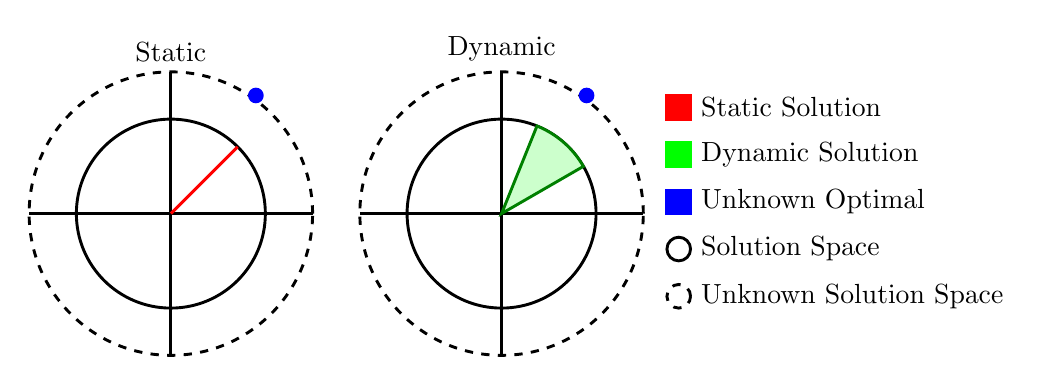
\begin{tikzpicture}[scale=0.6, line width=1.05][]

	\node at (0.0 , 1) [above] {Static};
    \draw (-3.0,  -2.0) -- ( 3.0,  -2.0);
	\draw ( 0.0, -5.0) -- ( 0.0,  1.0);
	\draw ( 0.0,  -2.0) circle [radius=2cm];
	\draw[dashed] ( 0.0,  -2.0) circle [radius=3.0cm];
	\node[blue] at (1.8, 0.5) [circle, fill, inner sep=2pt]{};
	\draw[red] (0.0, -2.0) -- ++(45:2.0);

	\node at (7.0 , 1) [above] {Dynamic};
    \draw ( 4.0,  -2.0) -- (10.0, -2.0);
	\draw ( 7.0, -5.0) -- ( 7.0, 1.0);
	\draw ( 7.0,  -2.0) circle [radius=2cm];
	\draw[dashed] ( 7.0,  -2.0) circle [radius=3.0cm];
	\node[blue] at (8.8, 0.5) [circle, fill, inner sep=2pt]{};
	\filldraw[fill=green!20,draw=green!50!black] (7,-2) -- ++(30:2.cm)
	        arc [start angle=30, end angle=68, radius=2.cm] -- cycle;

	
	\begin{scope}[shift={(10.5,0.5)}]
		% \node at (-0.25,1) [right] {};
		\draw[color=red,fill] (0,0.0)  rectangle  (0.5, -0.5);
		\node[anchor=west] at (0.5, -0.25) { Static Solution };

		\draw[color=green,fill] (0,-1.0)  rectangle  (0.5, -1.5);
		\node[anchor=west] at (0.5, -1.25) { Dynamic Solution };

		\draw[color=blue,fill] (0,-2.0)  rectangle  (0.5, -2.5);
		\node[anchor=west] at (0.5, -2.25) { Unknown Optimal };

		\draw[color=black] (0.25,-3.25)  circle  (0.25);
		\node[anchor=west] at (0.5, -3.25) { Solution Space };

		\draw[color=black,dashed] (0.25,-4.25)  circle  (0.25);
		\node[anchor=west] at (0.5, -4.25) { Unknown Solution Space };

		
	\end{scope}

    % \shade[ball color=red!50!white,opacity=0.8] (0,0) -- (90:\radius) arc (90:-90:\height) -- cycle;

	\end{tikzpicture}
}


			\drawReactiveConstraints{}

		\begin{itemize}
			\item Mathematical models guide direction but does not provide direct solutions.
			\item Static solutions are rarely fully executable.
			\item Dynamic models are less constrained and ensure a contained optimal solution.
			\item Remember: The real optimal solution is ever knowable at time = 0
		\end{itemize}
    \end{block}
\end{frame}

\begin{frame}[t]{}
    \begin{block}{Dynamic }
    \end{block}
\end{frame}

\begin{frame}[t]{}
    \begin{block}{}
		\input{../../figures/metaheuristic_understanding/quality-versus-time.tex}
    \end{block}
\end{frame}

\begin{frame}{}
    \begin{block}{Business}
		% Business usually handle decision making by making a series of "model changes" which 
		% are then combined to create a decision process.
  %       \begin{enumerate}
  %       \end{enumerate}
    \end{block}
\end{frame}

\end{document}
